
\section{Non-homogeneous Poisson Process}

The account selected for the extraction of the tweets is \textit{@realmadrid} since it has a constant number of retweets (RT), not extremely high, allowing us to measure the counting process in a reasonable time space. Although library \textit{rtweet} obtains information about the retweets and their time stamps it is worth mentioning that the results detailed here do not reflect the actual behaviour of the account since retweet count is limited to 100.

\subsection{Use descriptive statistics and graphics to explore the retweets data set in terms of the number of retweets by time and the time between retweets. Does it fit the hypothesis of a Poisson process?}

We know that a Poisson process is a counting process related with the Poisson and Exponential distributions. Being a counting process a stochastic process $\mathbf{N} = \{ N_t, t \geq 0 \}$ satisfying:
\begin{itemize}
	\item $N_t=0$
	\item $N_t$ is integer valued
	\item For $s<t, N_s \leq N_t$
	\item For $s<t, N_t - N_s$ represents the number of events that occur in the time intervals (s, t]
\end{itemize}

When plotting the tweet with maximum retweets (limited) we can see the behaviour of the retweet counting process.
\begin{figure}[H]
	\centering
	% Created by tikzDevice version 0.12.3 on 2019-12-17 19:18:25
% !TEX encoding = UTF-8 Unicode
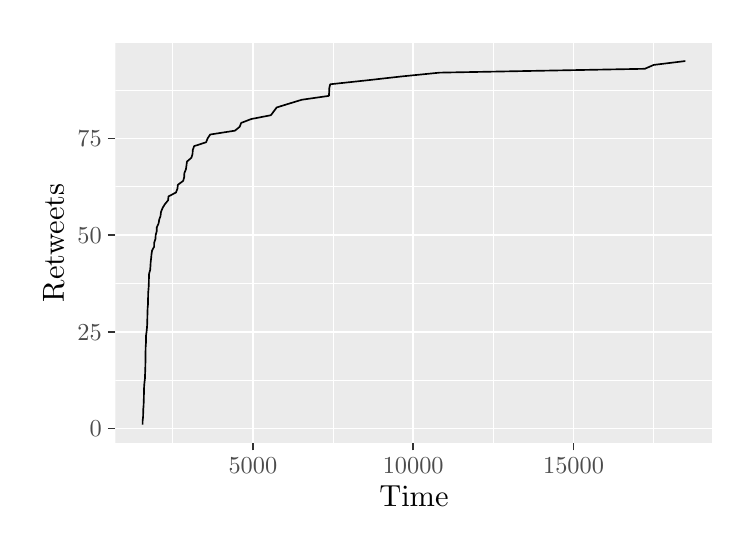
\begin{tikzpicture}[x=1pt,y=1pt]
\definecolor{fillColor}{RGB}{255,255,255}
\path[use as bounding box,fill=fillColor,fill opacity=0.00] (0,0) rectangle (252.94,180.67);
\begin{scope}
\path[clip] (  0.00,  0.00) rectangle (252.94,180.67);
\definecolor{drawColor}{RGB}{255,255,255}
\definecolor{fillColor}{RGB}{255,255,255}

\path[draw=drawColor,line width= 0.6pt,line join=round,line cap=round,fill=fillColor] (  0.00,  0.00) rectangle (252.94,180.68);
\end{scope}
\begin{scope}
\path[clip] ( 31.71, 30.69) rectangle (247.44,175.17);
\definecolor{fillColor}{gray}{0.92}

\path[fill=fillColor] ( 31.71, 30.69) rectangle (247.44,175.17);
\definecolor{drawColor}{RGB}{255,255,255}

\path[draw=drawColor,line width= 0.3pt,line join=round] ( 31.71, 53.32) --
	(247.44, 53.32);

\path[draw=drawColor,line width= 0.3pt,line join=round] ( 31.71, 88.26) --
	(247.44, 88.26);

\path[draw=drawColor,line width= 0.3pt,line join=round] ( 31.71,123.19) --
	(247.44,123.19);

\path[draw=drawColor,line width= 0.3pt,line join=round] ( 31.71,158.13) --
	(247.44,158.13);

\path[draw=drawColor,line width= 0.3pt,line join=round] ( 52.40, 30.69) --
	( 52.40,175.17);

\path[draw=drawColor,line width= 0.3pt,line join=round] (110.35, 30.69) --
	(110.35,175.17);

\path[draw=drawColor,line width= 0.3pt,line join=round] (168.29, 30.69) --
	(168.29,175.17);

\path[draw=drawColor,line width= 0.3pt,line join=round] (226.23, 30.69) --
	(226.23,175.17);

\path[draw=drawColor,line width= 0.6pt,line join=round] ( 31.71, 35.86) --
	(247.44, 35.86);

\path[draw=drawColor,line width= 0.6pt,line join=round] ( 31.71, 70.79) --
	(247.44, 70.79);

\path[draw=drawColor,line width= 0.6pt,line join=round] ( 31.71,105.73) --
	(247.44,105.73);

\path[draw=drawColor,line width= 0.6pt,line join=round] ( 31.71,140.66) --
	(247.44,140.66);

\path[draw=drawColor,line width= 0.6pt,line join=round] ( 81.37, 30.69) --
	( 81.37,175.17);

\path[draw=drawColor,line width= 0.6pt,line join=round] (139.32, 30.69) --
	(139.32,175.17);

\path[draw=drawColor,line width= 0.6pt,line join=round] (197.26, 30.69) --
	(197.26,175.17);
\definecolor{drawColor}{RGB}{0,0,0}

\path[draw=drawColor,line width= 0.6pt,line join=round] ( 41.52, 37.25) --
	( 41.55, 38.65) --
	( 41.70, 40.05) --
	( 41.74, 41.45) --
	( 41.77, 42.84) --
	( 41.90, 44.24) --
	( 41.93, 45.64) --
	( 41.99, 47.04) --
	( 42.01, 48.43) --
	( 42.03, 49.83) --
	( 42.09, 51.23) --
	( 42.22, 52.62) --
	( 42.39, 54.02) --
	( 42.42, 55.42) --
	( 42.48, 56.82) --
	( 42.52, 58.21) --
	( 42.55, 59.61) --
	( 42.55, 61.01) --
	( 42.56, 62.41) --
	( 42.60, 63.80) --
	( 42.63, 65.20) --
	( 42.73, 66.60) --
	( 42.74, 68.00) --
	( 42.76, 69.39) --
	( 42.96, 70.79) --
	( 43.11, 72.19) --
	( 43.19, 73.59) --
	( 43.23, 74.98) --
	( 43.25, 76.38) --
	( 43.32, 77.78) --
	( 43.33, 79.17) --
	( 43.46, 80.57) --
	( 43.46, 81.97) --
	( 43.52, 83.37) --
	( 43.54, 84.76) --
	( 43.66, 86.16) --
	( 43.76, 87.56) --
	( 43.79, 88.96) --
	( 43.82, 90.35) --
	( 43.87, 91.75) --
	( 44.26, 93.15) --
	( 44.37, 94.55) --
	( 44.45, 95.94) --
	( 44.61, 97.34) --
	( 44.74, 98.74) --
	( 44.95,100.14) --
	( 45.70,101.53) --
	( 45.71,102.93) --
	( 46.17,104.33) --
	( 46.25,105.73) --
	( 46.63,107.12) --
	( 46.66,108.52) --
	( 47.30,109.92) --
	( 47.54,111.31) --
	( 48.02,112.71) --
	( 48.18,114.11) --
	( 48.74,115.51) --
	( 49.59,116.90) --
	( 50.74,118.30) --
	( 50.88,119.70) --
	( 53.58,121.10) --
	( 54.12,122.49) --
	( 54.26,123.89) --
	( 56.18,125.29) --
	( 56.57,126.69) --
	( 56.61,128.08) --
	( 57.18,129.48) --
	( 57.38,130.88) --
	( 57.56,132.28) --
	( 59.16,133.67) --
	( 59.58,135.07) --
	( 59.66,136.47) --
	( 60.15,137.86) --
	( 64.48,139.26) --
	( 65.02,140.66) --
	( 65.95,142.06) --
	( 74.89,143.45) --
	( 76.61,144.85) --
	( 77.14,146.25) --
	( 80.76,147.65) --
	( 87.89,149.04) --
	( 88.93,150.44) --
	( 89.98,151.84) --
	( 94.51,153.24) --
	( 99.07,154.63) --
	(108.86,156.03) --
	(108.94,157.43) --
	(108.98,158.83) --
	(109.32,160.22) --
	(122.41,161.62) --
	(134.86,163.02) --
	(148.84,164.42) --
	(223.00,165.81) --
	(226.22,167.21) --
	(237.64,168.61);
\end{scope}
\begin{scope}
\path[clip] (  0.00,  0.00) rectangle (252.94,180.67);
\definecolor{drawColor}{gray}{0.30}

\node[text=drawColor,anchor=base east,inner sep=0pt, outer sep=0pt, scale=  0.88] at ( 26.76, 32.83) {0};

\node[text=drawColor,anchor=base east,inner sep=0pt, outer sep=0pt, scale=  0.88] at ( 26.76, 67.76) {25};

\node[text=drawColor,anchor=base east,inner sep=0pt, outer sep=0pt, scale=  0.88] at ( 26.76,102.69) {50};

\node[text=drawColor,anchor=base east,inner sep=0pt, outer sep=0pt, scale=  0.88] at ( 26.76,137.63) {75};
\end{scope}
\begin{scope}
\path[clip] (  0.00,  0.00) rectangle (252.94,180.67);
\definecolor{drawColor}{gray}{0.20}

\path[draw=drawColor,line width= 0.6pt,line join=round] ( 28.96, 35.86) --
	( 31.71, 35.86);

\path[draw=drawColor,line width= 0.6pt,line join=round] ( 28.96, 70.79) --
	( 31.71, 70.79);

\path[draw=drawColor,line width= 0.6pt,line join=round] ( 28.96,105.73) --
	( 31.71,105.73);

\path[draw=drawColor,line width= 0.6pt,line join=round] ( 28.96,140.66) --
	( 31.71,140.66);
\end{scope}
\begin{scope}
\path[clip] (  0.00,  0.00) rectangle (252.94,180.67);
\definecolor{drawColor}{gray}{0.20}

\path[draw=drawColor,line width= 0.6pt,line join=round] ( 81.37, 27.94) --
	( 81.37, 30.69);

\path[draw=drawColor,line width= 0.6pt,line join=round] (139.32, 27.94) --
	(139.32, 30.69);

\path[draw=drawColor,line width= 0.6pt,line join=round] (197.26, 27.94) --
	(197.26, 30.69);
\end{scope}
\begin{scope}
\path[clip] (  0.00,  0.00) rectangle (252.94,180.67);
\definecolor{drawColor}{gray}{0.30}

\node[text=drawColor,anchor=base,inner sep=0pt, outer sep=0pt, scale=  0.88] at ( 81.37, 19.68) {5000};

\node[text=drawColor,anchor=base,inner sep=0pt, outer sep=0pt, scale=  0.88] at (139.32, 19.68) {10000};

\node[text=drawColor,anchor=base,inner sep=0pt, outer sep=0pt, scale=  0.88] at (197.26, 19.68) {15000};
\end{scope}
\begin{scope}
\path[clip] (  0.00,  0.00) rectangle (252.94,180.67);
\definecolor{drawColor}{RGB}{0,0,0}

\node[text=drawColor,anchor=base,inner sep=0pt, outer sep=0pt, scale=  1.10] at (139.58,  7.64) {Time};
\end{scope}
\begin{scope}
\path[clip] (  0.00,  0.00) rectangle (252.94,180.67);
\definecolor{drawColor}{RGB}{0,0,0}

\node[text=drawColor,rotate= 90.00,anchor=base,inner sep=0pt, outer sep=0pt, scale=  1.10] at ( 13.08,102.93) {Retweets};
\end{scope}
\end{tikzpicture}

	\vspace*{-0.9em}
	\caption{Tweet with maximum RT process}
\end{figure}

Each retweet counting process is defined by a time series, measuring the time for the next count (in minutes) since the creation of the tweet. That is, starting at $N_t=0, t=0$ the arrival times $s$ increases the count by 1 unit.

Assuming that, if a user undoes a retweet, when acquiring the dataset the former time of retweet it is no longer recorded, the count can only increase and never decrease. The real model does not hold this assumption since this restriction is imposed by the internal functioning of Twitter and its API.

i.e. The following sequence of times would define a retweet counting process for a tweet with 6 RT. Where the first event occurs after 1.4 minutes.

\begin{center}
\textit{1.400000    1.616667    1.716667    1.716667    1.900000    2.616667}
\end{center}

Knowing that, as stated in Section 6.7 of Dobrow RP \textit{Introduction to Stochastic Processes with R}, a nonhomogeneous Poisson process is a counting process $(N_t)_{t\geq0}$ with intensity function $\lambda(t)$ if
\begin{itemize}
	\item $N_0 = 0$ 
	\item For all $t>0$, $N_t$ has a Poisson distribution with mean
	\[\mathbb{E}[N_t] = \int^t_0\lambda(x)dx\]
	\item For $0\leq q < r \leq s < t$, $N_r - N_q$ and $N_t - N_s$ are independent random variables.
\end{itemize}



\subsection{Assuming you can model the number of retweets by time as a non-homogeneous Poisson process with intensity function $ \lambda (t) = \theta e^{-\theta t},\ t>0$, graphically explore possible values of $\theta$ and choose the one that best fit your data. Explain all the considerations you make.}

\textbf{TODO by Ricardo que no tengo ni puta de lo que ha hecho}

\subsection{Write an R function to simulate data from a non-homogeneous Poisson process during a given time interval. Describe the inputs and outputs of your function.}

As stated in section 11.5.1 of Ross, Sheldon \textit{Introduction To Probability Models}, given $n$ events of a non-homogeneous Poisson process by time $T$ the $n$ event times are independent with a common density function
\[f(s) = \frac{\lambda(s)}{m(t)},\ 0<s<T, \quad m(T) = \int^T_0\lambda(s)ds\]

By simulating $N(T)$, the number of events by time T, and then simulating $N(T)$ random variables from the previous density function we can generate a NHPP.

\textbf{TODO Seguir explicando el algoritmo}

Translated into the following R function
\begin{lstlisting}[language=r]
simulateNHPP <- function(intensity_function, time, lambda_bound) {
	X <- numeric(0)
	
	for ( t in 1:time){
		u <- runif(2)
		accept <- u[2] <= intensity_function(time*u[1]) / lambda_bound
		if (accept)
			X <- c(X, time * u[1])
	}
		
	return(sort(X))
}
\end{lstlisting}
